\section{Testing}\label{Testing}
	This chapter will introduce our testing setup together with the result of our testing. We will start by introducing the testing suite, how the testing client works and we will also have a discussion about strengths and weaknesses of the system as a whole. Then we will introduce the actual tests and present our results. After you have read this chapter it should be clear to you how to setup the testing suite, how to replicate our tests and you should have an in depth view of our results. The result section will also contain a discussion on the weaknesses which have had an effect on the tests and how we have interpreted our results despite this.
    
    %% To be written, about the testing routines and NS3 and the test results. 
    
    \subsection{About the testing suite}\label{Testing:About}
        \subsubsection{Test Client}\label{Testing:About:Client}
            In this section we will shortly describe the test client used for testing, \ref{attachment?}"EchoClientClient.jar".
            % TODO: fix ref.

            The client starts by reading its configuration file. Its filename can be provided as the only command line argument, otherwise it defaults to "client.config'. This configuration file contains variables such as username, password, role, service to contact, what the request should be, how many requests to send and with what interval it should send them at, and some describing what to log.

            The client expects the request to contain '{REQID}' as part of the request message, and before sending it, the client will replace it with '{REQID=XX}' where 'XX' is the number of the request. This way the client can check that it gets the right response by checking whether '{REQID=XX}' is present in the response, and whether the ID is correct. This makes validating the response from the service easier, but it restricts the service to put the request message somewhere in the response. Another side effect of this being the only validation is that other errors in the response are not easily detected as long as the '{REQID=XX}' is there. If for example the response is cut short, by the stream being cut, as long as the ID is present it will be treated as valid. The client also prints the length of the response, so scripts that parse the results can pick up on responses with abnormal lengths.

            After reading the configuration file the client makes an instance of the client library\ref{some client library reference} 
            % TODO: fix ref.
            using the username, password and role, and itself as an ExceptionHandler. By implementing itself as the ExceptionHandler the client will be notified about all the exceptions ocurring in the client library, the client does not act upon these exceptions, but it does log them. A normal client might want to send a request again here.
            
            A timer is used to start the sending/receiving in a new thread at the interval specified and the number of times specified. Starting new threads for every request and sending at a small interval is a good way to test how the client library handles concurrent requests.

            The actual sending and receiving of data is rather simple, as you can see in this code snippet:
            \begin{figure}[h]
                \centering
                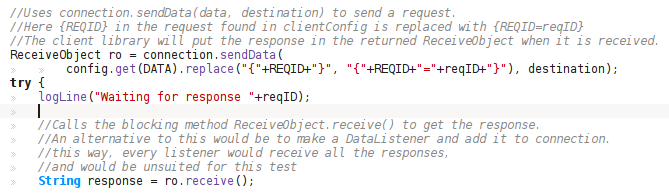
\includegraphics[width=\textwidth]{TestClientSending}
                \caption{Sending and Receiving in the Test Client}
                This code snippet shows how sending and receiving is done in the test client using the client library.
                \label{fig:TestClientSending}
            \end{figure}
            \\
            For more details about configuring the test client read the example configuration provided \ref{attachments:client.config}. For more detailed information on how the test client works, the java file with javadoc is provided \ref{attachments:TestClient.java}.
            % TODO: fix refs.

        \subsubsection{Test Service}\label{Testing:About:Service}
            In this section we will shortly describe the test service used for testing, \ref{attachment?}"EchoServiceLargeReply.war".
            % TODO: fix ref.

            The test service is very simple and deployable with GlassFish. It expects a request like this:
            \begin{figure}[h]
                \centering
                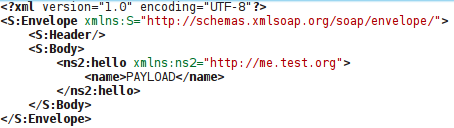
\includegraphics[width=\textwidth]{TestServiceRequest}
                \label{fig:TestServiceRequest}
            \end{figure}
            \\
            And responds like this:
            \begin{figure}[h]
                \centering
                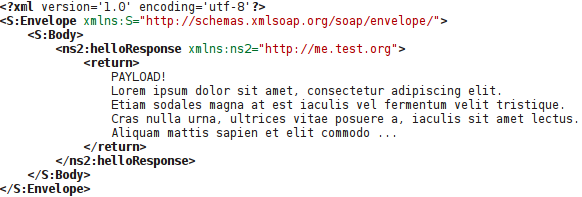
\includegraphics[width=\textwidth]{TestServiceResponse}
                \label{fig:TestServiceResponse}
            \end{figure}
            With PAYLOAD intact, and 10Kb of Lorem Ipsum\footnote{\URL{http://www.lipsum.com/} - simply dummy text}. We add these 10Kb's of text to ensure that the response is considerably larger than the request, which should get us more realistic results when testing. We also sends the original payload back so the test client can easily identify which request was responded to. Those 10Kb of text also has a large impact on testing, it means that on lower than 10KBps bandwidth all the messages can't be sent in time. We chose to have it this way because it would give us a predictable test and also some static configuration on the ESB could be configured with this in mind.

	\subsection{Test Cases}\label{Testing:Cases}
	As most of the tests below are quite alike the reasoning behind them are also quite like. The main difference between them are the “Timeout” which refer to the timeout the ESB uses. For more about the “Timeout” see \ref{Configuration of the ESB}.

	Since this project had somewhat of a research focus from the customers side we did not perform these test in order for us to validate our system. Instead we have run these tests to try and say something about the feasibility of the original question asked when we started. We will come back to this topic in the result section.

\begin{tabular}{| p{4cm} | p{8cm} |}\label{test:1}
       \hline
       ID & 1 \\
       \hline
       Description &  In this test what we are looking at is how our system behaves with a very low timeout, since we have full control over the message sizes sent in the test we know that this timeout will be too low on the lower bandwidths, but should perform much better on high bandwidths. \\
    \hline
    NS3 variables & Datarate: 1KBps,5KBps,10KBps,20KBps,40KBps \\
    \hline
    ESB variables & \textbf{Timeout: 500} \\
    \hline
    Automated & \surd \\
    \hline
    Expected Result & We expect to see that the ESB will preempt even higher priority messages in the lower bandwidth tests because of the low timeout, but on higher bandwidths the sending time of the all the messages should be lower than on the later tests. To put that in the same setting as our results, we expect the percentage of successfully received messages to be lower than in the tests below, but we expect the time to also be lower across the board.  \\
    \hline
\end{tabular}
\\ \vdots \\
\begin{tabular}{| p{4cm} | p{8cm} |}\label{test:2}
       \hline
       ID & 2 \\
       \hline
       Description & In this test we have increased the timeout substantially, we expect to see some improvements on 10KBps and still retain some of the benefits of a lower timeout on 20- and 40KBps \\
       \hline
    NS3 variables & Datarate: 1KBps,5KBps,10KBps,20KBps,40KBps \\
    \hline
    ESB variables & \textbf{Timeout: 1000} \\
    \hline
    Automated & \surd \\
    \hline
    Expected Result & We expect to have a higher percentage of completed messages on 10KBps than with a timeout of 500 and we expect the results on 1-, 20- and 40KBps to be relatively unchanged. \\
    \hline
\end{tabular}
\\ \vdots \\
\begin{tabular}{| p{4cm} | p{8cm} |}\label{test:3}
       \hline
       ID & 3 \\
       \hline
       Description & Again we have increased the timeout and expect to see some improvements on percentage, but we the total time taken should start to drop on higher bandwidths.  \\
       \hline
    NS3 variables & Datarate: 1KBps,5KBps,10KBps,20KBps,40KBps \\
    \hline
    ESB variables & \textbf{Timeout: 2000} \\
    \hline
    Automated & \surd \\
    \hline
    Expected Result & We expect all the messages on 20 and 40KBps to arrive, we expect that on 10KBps more messages should arrive, but not all. The time taken should again increase. \\
    \hline
\end{tabular}
\\ \vdots \\
\begin{tabular}{| p{4cm} | p{8cm} |}\label{test:4}
       \hline
       ID & 4 \\
       \hline
       Description & In this test we want to see how the ESB copes with a much larger timeout.  \\
       \hline
    NS3 variables & Datarate: 1KBps,5KBps,10KBps,20KBps,40KBps \\
    \hline
    ESB variables & \textbf{Timeout: 5000} \\
    \hline
    Automated & \surd \\
    \hline
    Expected Result & We expect that 10-, 20- and 40KBps should be enough to get most of the messages for the high priority client through, the time taken should again increase and this should be noticeable on 40KBps compared to \ref{test:1}.  \\
    \hline
\end{tabular}
\\ \vdots \\
\begin{tabular}{| p{4cm} | p{8cm} |}\label{test:5}
       \hline
       ID & 5 \\
       \hline
       Description & In this test we have gone all out. The timeout is massivly increased to see how the ESB behaves on the lowest bandwidths, 1- and 5KBps respectively.  \\
       \hline
    NS3 variables & Datarate: 1KBps,5KBps,10KBps,20KBps,40KBps \\
    \hline
    ESB variables & \textbf{Timeout: 100 000} \\
    \hline
    Automated & \surd \\
    \hline
    Expected Result & We expect the same percentage on 10-, 20- and 40KBps as \ref{test:4}. What we want to see is that on 5KBps the percentage is increased quite substantially compared to the previous tests. \\
    \hline
\end{tabular}
    % test cases.
    % test results.
    % test setup
